\documentclass[tikz,border=6pt]{standalone}
\usepackage[utf8]{inputenc}
\usepackage{amsmath}
\usepackage{xcolor}
\usetikzlibrary{arrows.meta,calc}
\definecolor{azul}{HTML}{1E3A8A}
\definecolor{rojo}{HTML}{DC2626}
\definecolor{verde}{HTML}{16A34A}
\definecolor{gris}{HTML}{64748B}
\definecolor{violeta}{HTML}{7C3AED}
\definecolor{naranja}{HTML}{F59E0B}
\begin{document}
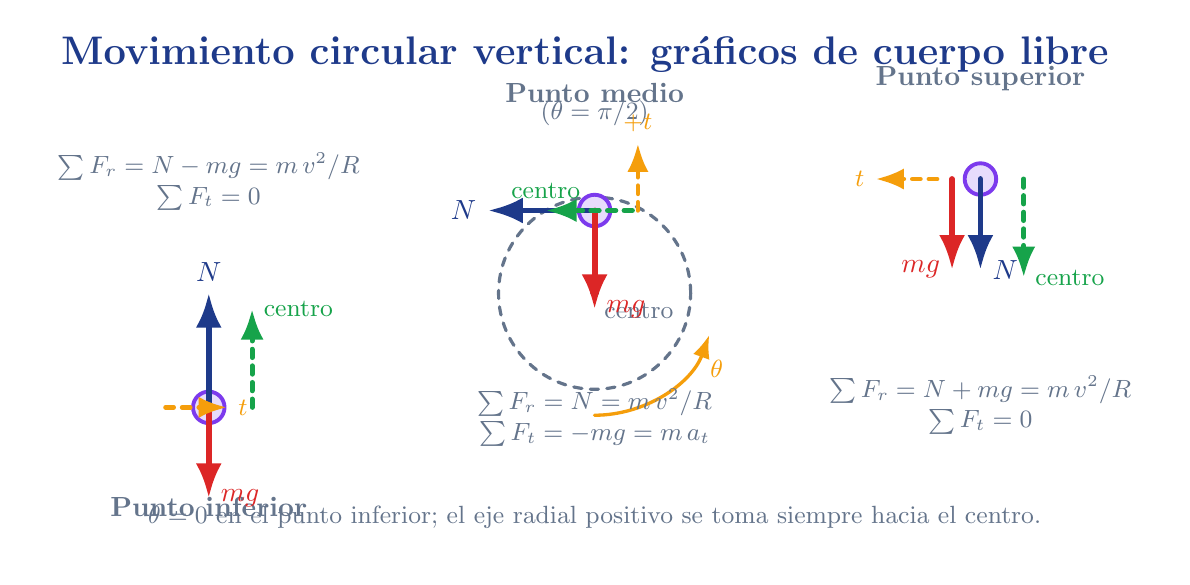
\begin{tikzpicture}[>=Latex, line cap=round, line join=round, font=\sffamily]
  \fill[white] (-7.2,-3.35) rectangle (7.2,3.35);
  \node[azul, font=\bfseries\Large, anchor=west] at (-6.9,3.03) {Movimiento circular vertical: gráficos de cuerpo libre};

  % Trayectoria de referencia
  \draw[gris, dashed, line width=1.15pt] (0,0) circle (1.22);
  \fill[black] (0,0) circle (1.5pt) node[below right, font=\small, text=gris] {centro};

  % Convención angular
  \draw[->, naranja, line width=1.2pt] (0,-1.55) arc[start angle=-90, end angle=-20, radius=1.55];
  \node[naranja, font=\small] at (1.55,-0.96) {$\theta$};
  \node[align=center, text=gris, font=\small] at (0,-2.85) {$\theta=0$ en el punto inferior; el eje radial positivo se toma siempre hacia el centro.};

  % Punto inferior
  \coordinate (B) at (-4.9,-1.45);
  \node[font=\bfseries, text=gris] at (-4.9,-2.72) {Punto inferior};
  \draw[violeta, fill=violeta!18, line width=1.4pt] (B) circle (0.20);
  \draw[->, azul, line width=2.1pt] (B) -- ++(0,1.45) node[above] {$N$};
  \draw[->, rojo, line width=2.1pt] (B) -- ++(0,-1.15) node[right] {$mg$};
  \draw[->, verde, dashed, line width=1.8pt] ($(B)+(0.55,0)$) -- ++(0,1.25) node[right, font=\small] {centro};
  \draw[->, naranja, dashed, line width=1.6pt] ($(B)+(-0.55,0)$) -- ++(0.78,0) node[right, font=\small] {$t$};
  \node[align=center, font=\small, text=gris] at (-4.9,1.42) {$\sum F_r=N-mg=m\,v^2/R$\\$\sum F_t=0$};

  % Punto medio lateral derecho
  \coordinate (M) at (0,1.05);
  \node[font=\bfseries, text=gris] at (0,2.55) {Punto medio};
  \node[font=\small, text=gris] at (0,2.28) {$(\theta=\pi/2)$};
  \draw[violeta, fill=violeta!18, line width=1.4pt] (M) circle (0.20);
  \draw[->, azul, line width=2.1pt] (M) -- ++(-1.35,0) node[left] {$N$};
  \draw[->, rojo, line width=2.1pt] (M) -- ++(0,-1.25) node[right] {$mg$};
  \draw[->, verde, dashed, line width=1.8pt] ($(M)+(0.48,0)$) -- ++(-1.10,0) node[above, font=\small] {centro};
  \draw[->, naranja, dashed, line width=1.6pt] ($(M)+(0.55,0)$) -- ++(0,0.85) node[above, font=\small] {$+t$};
  \node[align=center, font=\small, text=gris] at (0,-1.58) {$\sum F_r=N=m\,v^2/R$\\$\sum F_t=-mg=m\,a_t$};

  % Punto superior
  \coordinate (T) at (4.9,1.45);
  \node[font=\bfseries, text=gris] at (4.9,2.72) {Punto superior};
  \draw[violeta, fill=violeta!18, line width=1.4pt] (T) circle (0.20);
  \draw[->, azul, line width=2.1pt] (T) -- ++(0,-1.15) node[right] {$N$};
  \draw[->, rojo, line width=2.1pt] ($(T)+(-0.36,0)$) -- ++(0,-1.15) node[left] {$mg$};
  \draw[->, verde, dashed, line width=1.8pt] ($(T)+(0.55,0)$) -- ++(0,-1.25) node[right, font=\small] {centro};
  \draw[->, naranja, dashed, line width=1.6pt] ($(T)+(-0.55,0)$) -- ++(-0.78,0) node[left, font=\small] {$t$};
  \node[align=center, font=\small, text=gris] at (4.9,-1.42) {$\sum F_r=N+mg=m\,v^2/R$\\$\sum F_t=0$};
\end{tikzpicture}
\end{document}
